
\begin{figure}[t]
\vspace{-0.4cm}
\centering
\begin{tabular}{|c|c|}
\hline
 \multicolumn{2}{|c|} {\bf Time taken to converge} \\
\hline
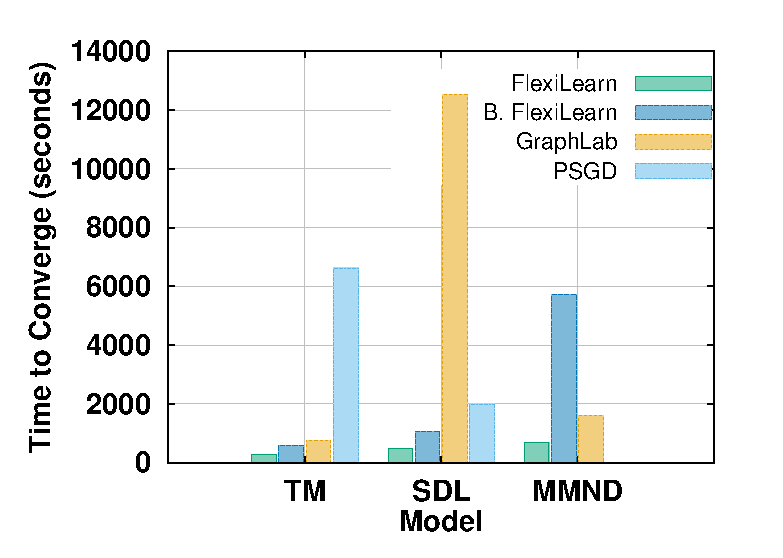
\includegraphics[width=0.46\columnwidth]{fig2/speedup.eps} &
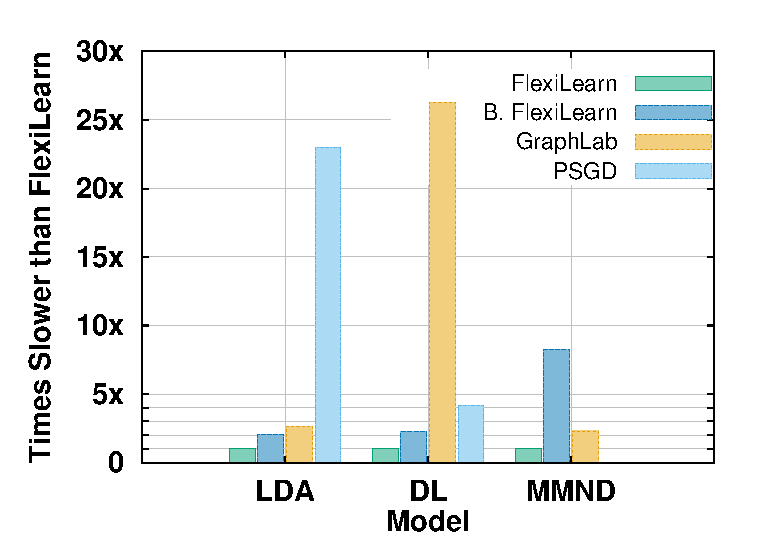
\includegraphics[width=0.46\columnwidth]{fig2/speedup2.eps} \\\hline
\end{tabular}
\vspace{-0.3cm}
\caption{\small Time taken by all methods to converge on the
three ML models, on an absolute scale (left) as well as a relative scale (right).
The methods plateau at these values in the respective plots shown
in figure~\ref{fig:results}. The bar for \psgd is absent in the figure as it never reaches $0.059$ and stops around 
objective value $0.092$.  }
\label{fig:speed}
\end{figure}

All four learning \schemes are evaluated on ithree criteria: 1) their speed, 2) scalability (in data size as well as 
model size), and 3) quality of answers. We see that \ourmethod outperforms all 
other schemes with huge margins on all three \queries \abhi{we call the three models as 
queries} and over all three criteria.


\subsection{Scalability}
Columns two, three and four in figure~\ref{fig:results} show the scalability of different
methods in model size, number of machines and data size for all three \queries. We can see
that \ourmethod performs quite well across the spectrum. 

%\vspace{-0.4cm}
%\section{Experiments}
%\vspace{-0.3cm}
%
%\begin{figure*}[t]
%\vspace{-0.4cm}
%\centering
%\begin{tabular}{|c|c|c|c|}
%\hline
%\multicolumn{2}{|c|}{\bf Topic Modeling} & {\bf Dictionary Learning} & {\bf MMND} \\
%\hline
%Convergence Plots & Scaling in \# Cores & Convergence Plots &  Convergence Plots \\
%%\multicolumn{4}{|c|}{\bf Topic Modeling} \\
%%\hline
%%Convergence Plots & \# of Topics & \# of Processors & \# of Docs \\
%\hline
%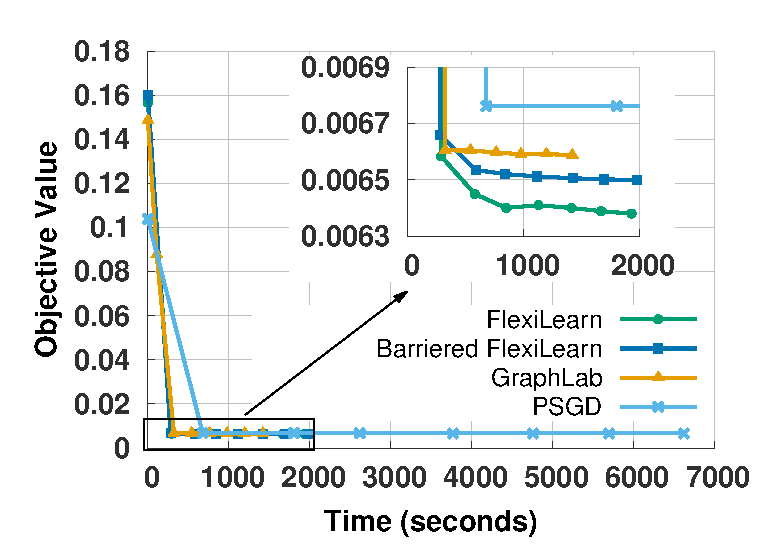
\includegraphics[width=0.23\textwidth]{fig2/lda_convergence.eps} 
%& 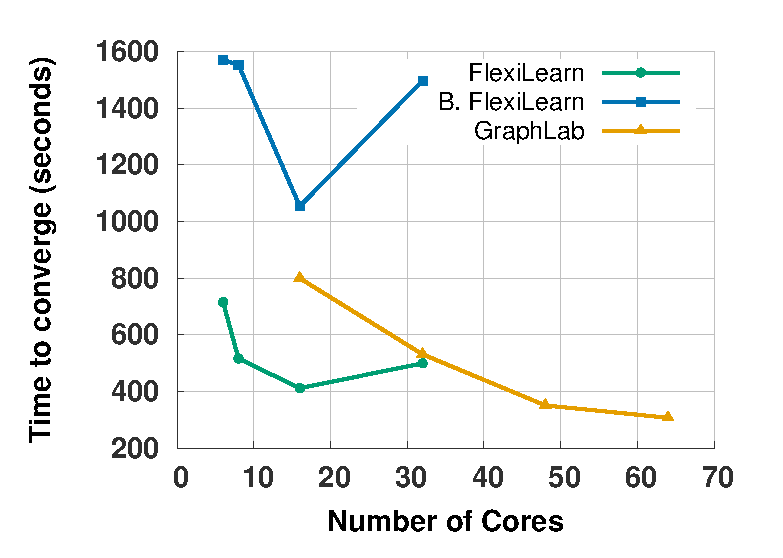
\includegraphics[width=0.23\textwidth]{fig2/lda_machines.eps} 
%& 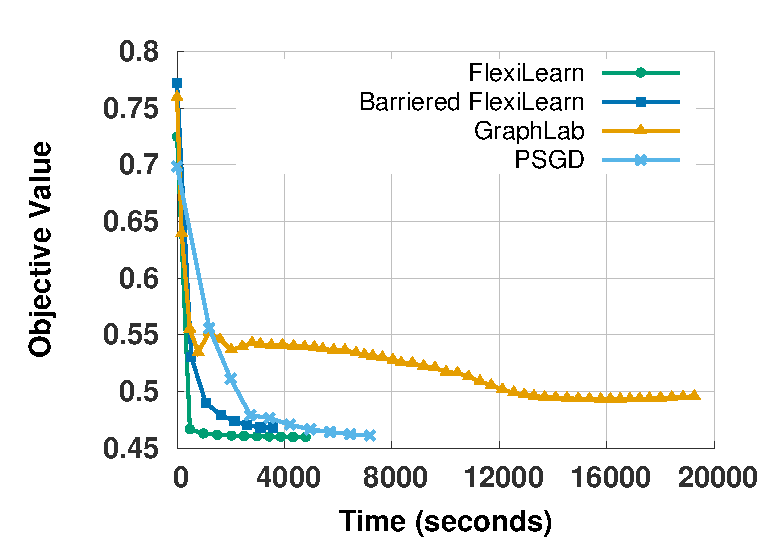
\includegraphics[width=0.23\textwidth]{fig2/dict_convergence.eps} 
%& 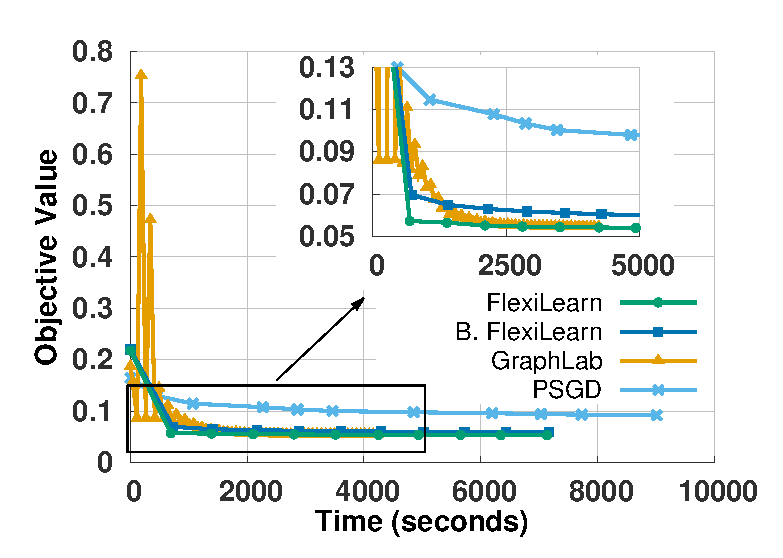
\includegraphics[width=0.23\textwidth]{fig2/mmsb_convergence.eps}  
%\\
%\hline
%%{\bf Topic Modeling} & {\bf Dictionary Learning} & \multicolumn{2}{|c|}{\bf Mixed Membership Network Decomposition} \\
%\multicolumn{4}{|c|}{\bf Topic Modeling} \\
%\hline
%Machines Needed & Scaling in \# Docs & \multicolumn{2}{|c|}{Scaling in \# Topics} \\
%\hline
%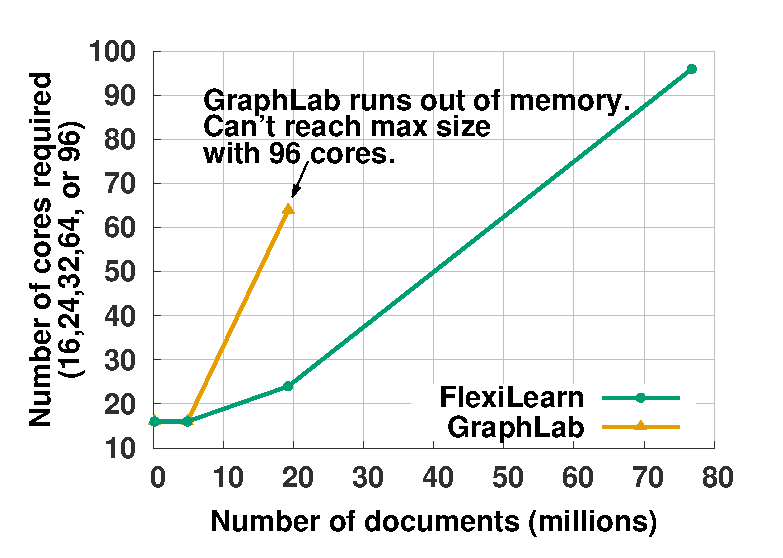
\includegraphics[width=0.23\textwidth]{fig2/lda_machines_failing.eps}
%& 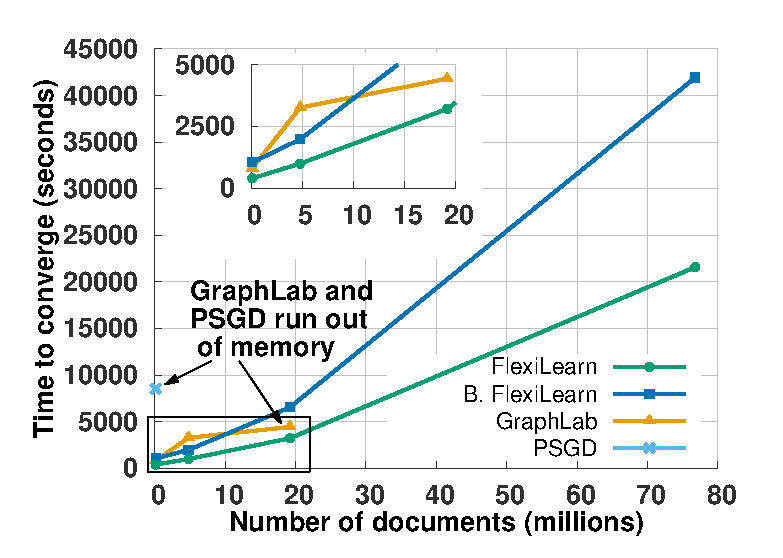
\includegraphics[width=0.23\textwidth]{fig2/lda_datasize.eps}
%& \multicolumn{2}{|c|}{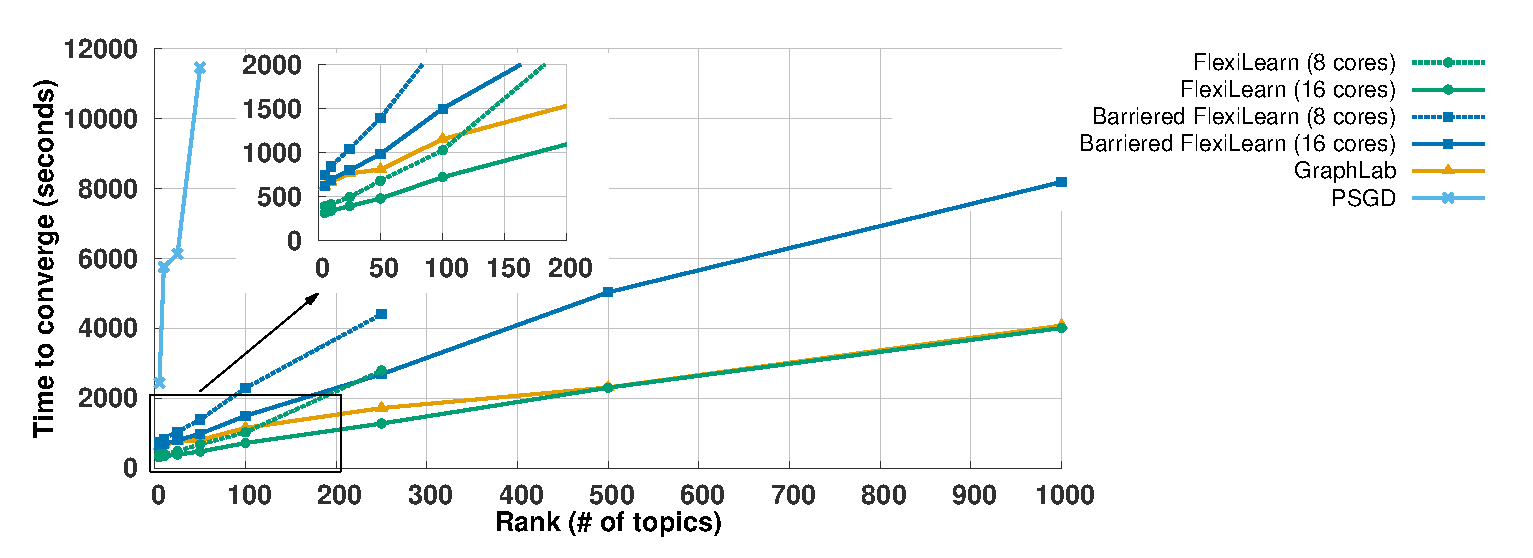
\includegraphics[width=0.46\textwidth]{fig2/lda_rankv2.eps}} \\
%\hline
%\end{tabular}
%\vspace{-0.3cm}
%\caption{\small Convergence and scalability plots for the three models (\lda, \dl, \mmsb),
%under our \ourmethod{} and baselines (\dsgd, \psgd, \graphlab). Unless otherwise stated in the plot, all methods were run with 16 cores
%and rank $K=25$. For all topic modeling plots except ``\# of Docs" and ``Machines Required", we used the NyTimes4 dataset (Table \ref{tab:dataset}).
%The convergence plots reveal the objective trajectory and final value of each method,
%while the scalability plots show how each method fares (on topic modeling) as we increase the problem rank, number of processor cores, and data size.
%In the bottom left, we also show the minimum number of machines required for a given topic modeling dataset size, for
%\ourmethod{} and \graphlab.}
%\vspace{-0.5cm}
%\label{fig:results}
%\end{figure*}

\paragraph{Dataset size}
Column four of figure~\ref{fig:results} shows the convergence time taken by the different
\schemes with respect to increasing data size. We vary the datasize in two ways: 1) by 
making the data denser e.g. increasing the number of words in a document in the 
topic modelling problem, 2) by increasing the dimensions of the data e.g. increasing the 
number of documents. In this set of experiments we vary the \lda and \sdl data 
size by increasing the number of documents. For \mmsb we increase the data by making it 
denser with inclusion of more edges as explained in section~\ref{subsec:data}. 
A subtle distinction between the two ways is that increasing the dimension of 
the data also increases the model sizei~\abhi{elaborate more as to why?}. 
This has negative repercussions for approaches
that are only scalable in data e.g. \psgd. We see that \psgd runs out of memory very early 
in the experiments for \lda and \sdl, but keeps running with increase in data for a 
while in case of \mmsb (although with poorer result quality and slower convergence) ~\abhi{get
\psgd results for \mmsb and \sdl asap}. Our \ourmethod scales well for both ways of increasing 
data size. It never runs out of memory in any of the \query types for sizes shown in the 
figure as well as is faster by atleast a factor of 2 usually. Figure~
\ref{fig:ldaMachinesNeeded} shows a comparison of number of machines needed for \ourmethod
and \graphlab for \lda. Figures~\ref{fig:results} and \ref{fig:ldaMachinesNeeded} that 
not only \ourmethod is faster but is also economic for a given data size.


\paragraph{Model parameters}
The model parameter are the types of variables that arise as a construct of the model (
section~\ref{subsec:abstractProblem}). For example, the number of topics 
in \lda or the number of basis vectors in \sdl is a construct of the model.  
Column two shows the variations for different models for increase in rank (topic, bases or
network role number). Here again we see that \ourmethod is faster to converge than all the other
approaches. The difference in convergence rate of \graphlab and \ourmethod is especially stark
for \sdl. The reason for this is that \graphlab oscillates by big margins for this \query as
seen in figure~\ref{fig:results}, second row, first column. 
\psgd runs out of memory quite early as expected for \lda and \sdl.
Since the dimensions of the \mmsb data are smaller (281,904) that \lda (1,200,000) or \sdl
(1,261,406), \psgd runs out of memory a little later for this \mmsb \query. 

\paragraph{Processors}
Column three shows the effects of varying number of processors for a fixed data and model size.
We have set rank as 25 and used \snytimes{N}, \swebgraph{N}, and \simagenet{N}
(\abhi{get the precise N value}) as data sets
for \lda, \mmsb, and \sdl. We see that for smaller datasizes the \ourmethod starts showing small
diminishing returns with increasing processors (\lda, column three, row one) and its curve
is worse than \graphlab. But for larger datasets (\mmsb, column three, row three), \ourmethod
has the best curve. This happens because for smaller datasest time taken to synchronize 
among the reducers dominates time taken to perform actual computations on the data. 
But compared to \ourmethod, \dsgd performs much worse (see \lda graph, column three,
row one). Our method due to its provably correct (\abhi{citations?}) always on property
mitigates the ill effects of synch-waits by doing more work.
Figure~\ref{fig:pieChart} shows a break up of the percentage of time each reducers
spend on various components of the task. ~\abhi{add more analysis here once the pie-chart is added}
\subsection{Convergence speed}
Figure~\ref{fig:speed} shows convergence times 
for \ourmethod{}, \dsgd, \psgd, and \graphlab over the three 
models: \lda, \mmsb and \dl. \ourmethod{} is faster
by anywhere between $2.6\times$ (vs \graphlab on \lda) 
to $26.2\times$ (vs \graphlab on \sdl). This clearly is due to the always-on 
property of \ourmethod.
%\begin{figure}[t]
%\vspace{-0.4cm}
%\centering
%\begin{tabular}{|c|c|}
%\hline
% \multicolumn{2}{|c|} {\bf Time taken to converge} \\
%\hline
%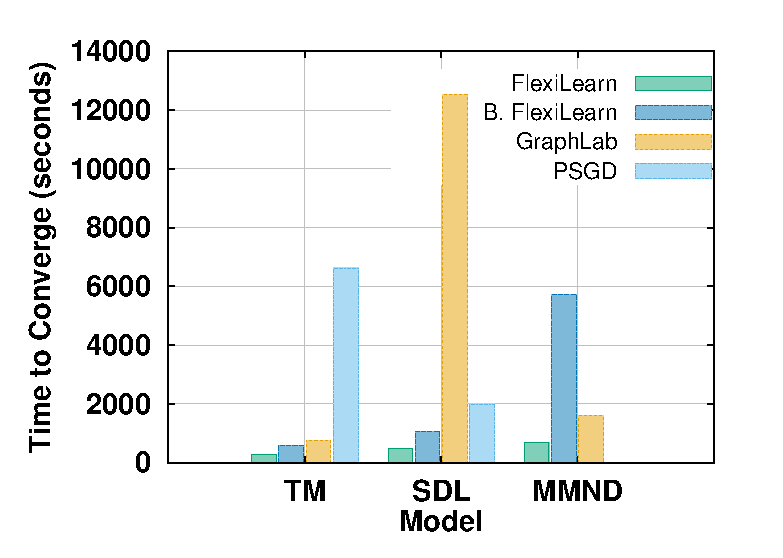
\includegraphics[width=0.46\columnwidth]{fig2/speedup.eps} &
%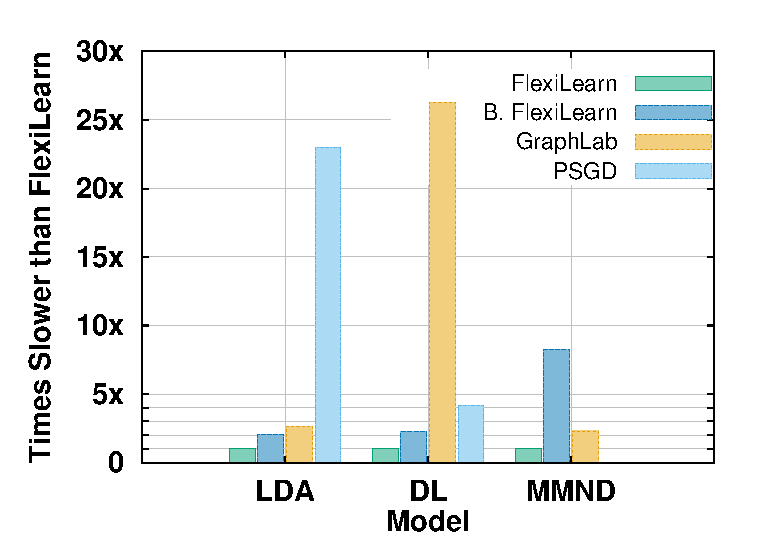
\includegraphics[width=0.46\columnwidth]{fig2/speedup2.eps} \\\hline
%\end{tabular}
%\vspace{-0.3cm}
%\caption{\small Time taken by all methods to converge on the
%three ML models, on an absolute scale (left) as well as a relative scale (right).
%The methods plateau at these values in the respective plots shown
%in figure~\ref{fig:results}. The bar for \psgd is absent in the figure as it never reaches $0.059$ and stops around 
%objective value $0.092$.  }
%\label{fig:speed}
%\end{figure}

\subsection{Convergence quality}
Though graphlab is large scale and is distributed work load system, it has no theoretical 
quarantees. This shows up in the quality of answers we get. \ourmethod is distributed, faster,
better scalable, and gives higher quelaity of answers. Figure~\ref{fig:results}, 
column one shows the convergence curve for all the approaches over all three \queries.
\ourmethod achieves better converegcen value with faster speed comapred to all other 
approaches. The higher quality of results stems from the fact that \ourmethod is 
theoretically sound. \graphlab oscialltes quite a lot for \mmsb and \sdl. This is due to  
the fact that it is picking up arbitrary vertices and updating them without any guarantees
for the constraints (as discussed in section~\ref{sec:complexQues})
%\graphlab oscillation reasons and patterns, \dsgd and \psgd converges to a poor
%quality,
\subsection{Why \ourmethod wins }
\ourmethod wins emphtically on all three criteria, and over all three \queries is due to 
follwoing salient properties:
\begin{itemize}
\item Unline \psgd, it is distributed over data as well as model. This gives \ourmethod 
atleast twice the speed as well as scalability compared to \psgd 
\item Unlike \graphlab, it is theoretically grounded. This gives \ourmethod a guarantee 
for high quality answers
\item Unline \dsgd it does not waste time while waiting to synchronize. This makes it 
more scalable (as we saw incase of machine scalability) and faster by several factors of
magnitude.
\end{itemize}
%Put a plot of waiting times in different concstraints case and argue why it
%helps here.
